\documentclass[11pt, oneside]{article}

%
% Packages
%

\usepackage{geometry}
\geometry{letterpaper}
\usepackage[parfill]{parskip}      		% Activate to begin paragraphs with an empty line rather than an indent
\usepackage{graphicx}
\usepackage{booktabs}
\usepackage{topcapt}
\usepackage[labelfont =  {sf, bf}, textfont = sf, format = plain]{caption}
\usepackage{amssymb}
\usepackage{amsmath}
\usepackage{natbib}
\usepackage{color}
\usepackage{array}
\usepackage{gensymb}
\usepackage{setspace}
\newcommand{\stretchy}{1.5}
\usepackage{lineno}

% Make helvetica the default sans-serif font
\renewcommand\sfdefault{phv}

% Package command for citing R packages
\newcommand{\pkg}[1]{{\fontseries{b}\selectfont #1}} 

%
% Commenting
%

\newcommand{\cdm}[1]{{ \color{magenta} [{\bf{CDM:}} {\em#1}]}} % Chris' comments are in magenta.
\newcommand{\ala}[1]{{ \color{blue} [{\bf{ALA:}} {\em#1}]}} % Amy's comments are in blue.

%
% Where to find files
%

\begin{knitrout}
\definecolor{shadecolor}{rgb}{0.969, 0.969, 0.969}\color{fgcolor}\begin{kframe}
\begin{alltt}
  \hlcom{# The path to the ms directory may need to be changed for different users}
  \hlcom{# Manuscript files}
  \hlstd{pathMS} \hlkwb{<-} \hlstr{"~/Google Drive/CardLocalAdaptation/ms"} \hlcom{# Chris' MacBook}
  \hlcom{# pathMS <- "~/Documents/CardAdapt/ms" # Chris' Linux laptop}

  \hlcom{# Data files for paper}
  \hlstd{pathDat} \hlkwb{<-} \hlkwd{paste}\hlstd{(pathMS,} \hlstr{"/Data"}\hlstd{,} \hlkwc{sep} \hlstd{=} \hlstr{""}\hlstd{)}

  \hlcom{# Figures for paper}
  \hlstd{pathFig} \hlkwb{<-} \hlkwd{paste}\hlstd{(pathMS,} \hlstr{"/Figures"}\hlstd{,} \hlkwc{sep} \hlstd{=} \hlstr{""}\hlstd{)}

  \hlcom{# Tables for paper}
  \hlstd{pathTab} \hlkwb{<-} \hlkwd{paste}\hlstd{(pathMS,} \hlstr{"/Tables"}\hlstd{,} \hlkwc{sep} \hlstd{=} \hlstr{""}\hlstd{)}

  \hlcom{# Small function to make statistical significance asterisks}
  \hlstd{sigStar} \hlkwb{<-} \hlkwa{function}\hlstd{(}\hlkwc{pvalue}\hlstd{)}
  \hlstd{\{}
    \hlkwa{if} \hlstd{(pvalue} \hlopt{>=} \hlnum{0.05}\hlstd{)} \hlkwd{return}\hlstd{(}\hlstr{""}\hlstd{)}
    \hlkwa{if} \hlstd{(pvalue} \hlopt{<} \hlnum{0.05} \hlopt{&} \hlstd{pvalue} \hlopt{>=} \hlnum{0.01}\hlstd{)} \hlkwd{return}\hlstd{(}\hlstr{"*"}\hlstd{)}
    \hlkwa{if} \hlstd{(pvalue} \hlopt{<} \hlnum{0.01} \hlopt{&} \hlstd{pvalue} \hlopt{>=} \hlnum{0.001}\hlstd{)} \hlkwd{return}\hlstd{(}\hlstr{"**"}\hlstd{)}
    \hlkwa{if} \hlstd{(pvalue} \hlopt{<} \hlnum{0.001}\hlstd{)} \hlkwd{return}\hlstd{(}\hlstr{"***"}\hlstd{)}
  \hlstd{\}}

  \hlcom{# Color palette}
  \hlcom{# Primary color:}

   \hlstd{primShade0} \hlkwb{<-} \hlkwd{rgb}\hlstd{(}\hlnum{1}\hlstd{,} \hlnum{0}\hlstd{,} \hlnum{0.286}\hlstd{)}
   \hlstd{primShade1} \hlkwb{<-} \hlkwd{rgb}\hlstd{(}\hlnum{1}\hlstd{,} \hlnum{0.643}\hlstd{,} \hlnum{0.745}\hlstd{)}
   \hlstd{primShade2} \hlkwb{<-} \hlkwd{rgb}\hlstd{(}\hlnum{1}\hlstd{,} \hlnum{0.439}\hlstd{,} \hlnum{0.6}\hlstd{)}
   \hlstd{primShade3} \hlkwb{<-} \hlkwd{rgb}\hlstd{(}\hlnum{0.765}\hlstd{,} \hlnum{0}\hlstd{,} \hlnum{0.22}\hlstd{)}
   \hlstd{primShade4} \hlkwb{<-} \hlkwd{rgb}\hlstd{(}\hlnum{0.588}\hlstd{,} \hlnum{0}\hlstd{,} \hlnum{0.169}\hlstd{)}

  \hlcom{# Secondary color (1):}

  \hlstd{sec1shade0} \hlkwb{<-} \hlkwd{rgb}\hlstd{(}\hlnum{0.008}\hlstd{,} \hlnum{0.957}\hlstd{,} \hlnum{1}\hlstd{)}
  \hlstd{sec1shade1} \hlkwb{<-} \hlkwd{rgb}\hlstd{(}\hlnum{0.643}\hlstd{,} \hlnum{0.984}\hlstd{,} \hlnum{1}\hlstd{)}
  \hlstd{sec1shade2} \hlkwb{<-} \hlkwd{rgb}\hlstd{(}\hlnum{0.443}\hlstd{,} \hlnum{0.976}\hlstd{,} \hlnum{1}\hlstd{)}
  \hlstd{sec1shade3} \hlkwb{<-} \hlkwd{rgb}\hlstd{(}\hlnum{0}\hlstd{,} \hlnum{0.49}\hlstd{,} \hlnum{0.514}\hlstd{)}
  \hlstd{sec1shade4} \hlkwb{<-} \hlkwd{rgb}\hlstd{(}\hlnum{0}\hlstd{,} \hlnum{0.376}\hlstd{,} \hlnum{0.396}\hlstd{)}

  \hlcom{# Secondary color (2):}

  \hlstd{sec2shade0} \hlkwb{<-} \hlkwd{rgb}\hlstd{(}\hlnum{0.988}\hlstd{,} \hlnum{1}\hlstd{,} \hlnum{0}\hlstd{)}
  \hlstd{sec2shade1} \hlkwb{<-} \hlkwd{rgb}\hlstd{(}\hlnum{0.996}\hlstd{,} \hlnum{1}\hlstd{,} \hlnum{0.643}\hlstd{)}
  \hlstd{sec2shade2} \hlkwb{<-} \hlkwd{rgb}\hlstd{(}\hlnum{0.992}\hlstd{,} \hlnum{1}\hlstd{,} \hlnum{0.439}\hlstd{)}
  \hlstd{sec2shade3} \hlkwb{<-} \hlkwd{rgb}\hlstd{(}\hlnum{0.835}\hlstd{,} \hlnum{0.847}\hlstd{,} \hlnum{0}\hlstd{)}
  \hlstd{sec2shade4} \hlkwb{<-} \hlkwd{rgb}\hlstd{(}\hlnum{0.643}\hlstd{,} \hlnum{0.651}\hlstd{,} \hlnum{0}\hlstd{)}
\end{alltt}
\end{kframe}
\end{knitrout}

%
% Title and authors
%

\title{(working title) Local Physiological Adaptation in \textit{Mimulus cardinalis}}
\author{Christopher D. Muir and Amy L. Angert}
%\date{}							% Activate to display a given date or no date

%
% Start document
%

\begin{document}
\maketitle
\listoffigures
\listoftables

\section*{Abstract}

\setstretch{\stretchy}

\section*{Introduction}

% Toggle these commands to get version for doing word count
\linenumbers
%\pagenumbering{gobble}
%\raggedright

Local adaptation is one of the most ubiquitous observations in nature: organisms perform well in their natal environment, but poorly outside it. Local adaptation within species most often involves genetic differences in ecologically relevant traits caused by selection to different environments, leading to predictable trait-environment correlations that persist in a common garden. Although local adaptation is well-supported by data from reciprocal transplant experiments, trait-environment associations, and ecological genetics/genomics, predicting which traits respond to selection exceeds our understanding. In particular, the role of physiological traits is poorly understood, even though physiology explains adaptation to the abiotic environment, which we need to understand as a baseline for anticipating how organisms will respond to climate change. A related problem is identifying the exact selective agents, such as abiotic factors like soil water availability or biotic interactions [etc.]... Here, we simultaneously investigate which traits and causal selective agents explain range-wide patterns of local physiological adaptation to climate in \textit{Mimulus}, a model genus for local adaptation studies.

% niche-tracking versus niche-shifting
One surprising pattern is that populations adapt to different environments by adjusting their life history to stay within the same fundamental physiological niche rather than have the niche itself evolve. For example, mosquitoes adjust diapause length with latitude rather than evolve altered ...\cdm{what other examples could we include here?} This suggests that in many situations it is evolutionarily easier to change life history rather than fundamental physiological tolerance.

% Selective agents
We also know little about the selective agents, such as climatic factors or biotic interactions, that are most important in driving adaptive divergence. In certain situations, such as pollinator shifts and edaphic adaptation, it is straightforward to identify putative selective agents and test predicted mechanisms. However, it is more challenging for cases in which traits vary with less specific factors like mean annual precipitation or latitude. For example, body size clines (larger size at higher latitude) have evolved repeatedly on three contients in \textit{Drosophila subobscura}, strongly indicating selection. But which one or more of the many climatic factors that covary with latitude actually controls selection on body size? Selection might be even more complex for species that live over multiple seasons, meaning that environmental variation rather than the average environment may be a selective agent.

% Motivate using Mimulus
Linking physiological traits to potentially complex patterns of local adaptation requires integrating multiple lines of evidence from comparative, experimental, genomic studies under both lab and field conditions. Many classic and contemporary studies of local adaptation have been conducted using species from genus \textit{Mimulus} because of its natural history, easy propogation, and genetic/genomic resources. ... Conspicuous absence of phys mechanism

% Final paragraph
1. `intrinsic' physiological variation
2. variation in plasticity
3. what ecological factors explain divergence (i.e. putative selective agents underlying local adaptation)

Conclude that observations are best explained by stabilizing selection on the fundamental niche, but spatially varying divergent selection on coordinated life history and physiological traits.

\section*{Methods}

\subsection*{Population Selection}

We used 16 populations from throughout the range of \textit{M. cardinalis} (Table 1). Seeds were collected in the field \cdm{Amy, can you explain seed collection methods?}.



\begin{table}[ht]
   \centering
   \topcaption{16 Focal populations}
   \begin{tabular}{@{} lllllll @{}}
      \toprule
  Name& Region  & Demo?& Pop gen?& Latitude  & Longtiude  & Elevation (mas) \\
      \midrule
	HAU & South Margin		& yes	& yes	& 	& 
    	&    \\
	CTC	& South Margin		& yes	& no	&  & 
    	&    \\
	CUR	& South Margin		& yes	& yes &  & 
    	&    \\
	GRP & South Margin		& no	& no	&  &
    	&    \\
	WWC &	Transverse		  & yes	& yes	&  & 
    	&    \\
	MIL	& Transverse	  	& yes	& no	&  & 
    	&    \\
	WFM	& Transverse	  	& yes	& no	&  & 
    	&    \\
	NMT	& South Sierras		& yes	& yes?&  & 
    	&    \\
	PRD	& South Sierras		& yes	& yes	&  & 
    	&    \\
	RWD	& South Sierras		& yes	& yes	&  & 
    	&    \\
	WNA	& Central Sierras	& yes	& yes	&  & 
    	&    \\
	RBW	& Central Sierras	& yes	& no	&  & 
    	&    \\
	MYU	& North Sierras		& yes	& yes	&  & 
    	&    \\
	LIJ	& North Sierras		& yes	& yes	&  & 
    	&    \\
	DPC	& North Coast	  	& yes	& yes	&  & 
    	&    \\
	RCC	& North Margin		& yes	& yes	&  & 
    	&    \\
	\bottomrule
   \end{tabular}
\end{table}

\subsection*{Plant propagation}

On 14 April, 2014, 3-5 seeds per family were sown directly on sand (Quikrete Play Sand, Georgia, USA) watered to field capacity in RLC4 Ray Leach cone-tainers placed in RL98 98-well trays (Stuewe \& Sons, Inc., Oregon, USA). We used pure sand both to facilitate root-washing and because \textit{M. cardinalis} typically grows in sandy, riparian soils (A. Angert, pers. obs.). Two jumbo-sized cotton balls at the bottom of cone-tainers prevented sand from washing out. Cone-tainers were continuously bottom-watered during germination by placing them in medium-sized flow trays (FLOWTMD, Stuewe \& Sons, Inc., Oregon, USA) filled part way with water, placed on benches in greenhouses at the University British Columbia campus in Vancouver, Canada (49\degree 15' N, 123\degree 15' W). Misters thoroughly wetted the top of the sand every two hours during the day. Most seeds germinated between 1 and 2 weeks, but we allowed 3 weeks before transferring seedlings to growth chambers. Germination was recorded daily from one to two weeks after sowing, and every few days thereafter. On 5 May (21 days after sowing), seedlings were transferred to one of two MODEL Growth Chambers (Conviron, Manitoba, Canada). We thinned seedlings to one plant per cone-tainer, leaving the center-most plant. 702 of 768 (91.4\%) had plants that could be used in the experiment. We allowed one week at constant, non stressful conditions (day: 20\celsius, night: 16\celsius) for plants to acclimate to growth chambers before starting treatments. The initial size of seedlings, measured as the length of the first true leaves, did not differ between populations, families, or treatments (Table S\#).
    
\subsection*{Treatments}

We imposed four treatments, a fully-factorial cross of two temperature treatments and two watering treatments. Because growth chambers cannot be subdivided, one chamber was assigned to the Hot treatment and another to the Cool treatment. Within each chamber, there were two Well-watered blocks and two Drought blocks. A detailed description of treatments is given below \cdm{should some be moved to supplement?} and summarized in Fig~\ref{fig:Fig_ExptlDes}. The irradiance in both chambers was approximately 400 $\mu$mol quanta m$^{-2}$ s$^{-1}$. The growth chambers did not control humidity, but because of watering and high plant transpiration rates, the relative humidity was quite high in both temperature treatments (data not shown). 

\subsubsection*{Temperature treatments}

We simulated typical growing season (June 1 - August 15) air temperatures at the two most thermally divergent focal sites in our study, Whitewater Canyon (Hot) and Little Jameson (Cool). We downloaded daily interpolated mean, minimum, and maximum air temperature from 13 years (2000-2012) at both sites from ClimateWNA \citep{Wang_etal_2012}. Daily temperatures from ClimateWNA are highly correlated with the air temperature recorded from data loggers in the field at these sites (A. Angert, unpub. data). Hence, the ClimateWNA temperature profiles are similar to actual thermal regimes experienced by \textit{M. cardinalis} in nature. We simulated realistic temperature regimes by calculating the mean temperature trend from June to August using LOESS \citep{Cleveland_etal_1992}. The residuals were highly autocorrelated at both sites (warmer than average days are typically followed by more warm days) and there was strong correlation ($r = 0.65$) between sites (warm days in WWC were also warm in LIJ). The `VARselect' function in the \pkg{vars} package for R \citep{Pfaff_2008} indicated that a lag two Vector Autoregression (VAR(2)) model best captured the within-site autocorrelation as well as between-site correlation in residuals. We fit and simulated from the VAR(2) model using the package \pkg{dse} \citep{Gilbert_2014} in R. Simulated data closely resembled the autocorrelation and between-site correlation of the actual data. From simulated mean temperature, we next selected minimum and maximum daily temperatures. Mean, min, and max temperature were highly correlated at both sites. We chose min and max temperatures using site-specific fitted linear models between mean, max, and min temperature, with additional variation given by normally-distributed random deviates with variance equal to the residual variance of the linear models. For each day, the nighttime (22:00 - 6:00) chamber temperature was set to the simulated minimum temperature. During the middle of the day, temperature was set to the simulated maximum temperature, with a variable period of transition between min and max so that the average temperature was equal the simulated mean temperature.

\subsubsection*{Watering treatments}

For watering treatments, we simulated two extreme types of streams where \textit{M. cardinalis} grows. In the well-watered treatment, we simulated a large stream that never goes dry during the summer growing season. In the drought treatment, we simulated a small stream that has ample flow at the beginning of the season, but gradually dries down as the winter snow pack melts. In both treatments, plants were bottom-watered using  water chilled to 7.5 [check] by MAKE AND MODEL OF CHILLER. Plants in the well-watered treatment were fully saturated every two hours during the day. Watering in the drought treatment gradually declined from every two hours to every day between May 20 (36 days after sowing) and 10 June (57 days after sowing). Simultaneously, the amount of bottom-watering per flood decreased, such that only the bottom of the cone-tainers were wetted by the end of the experiment.

\cdm{Are there any data from California about soil water content through the season?}

\begin{knitrout}
\definecolor{shadecolor}{rgb}{0.969, 0.969, 0.969}\color{fgcolor}\begin{kframe}
\begin{alltt}
\hlkwd{library}\hlstd{(scales)} \hlcom{# for color transparency}
\hlstd{exptlDes} \hlkwb{<-} \hlkwd{read.csv}\hlstd{(}\hlkwd{paste}\hlstd{(pathDat,} \hlstr{"/ExperimentalDesign.csv"}\hlstd{,} \hlkwc{sep} \hlstd{=} \hlstr{""}\hlstd{))}

\hlkwd{pdf}\hlstd{(}\hlkwd{paste}\hlstd{(pathFig,} \hlstr{"/ExperimentalDesignBase.pdf"}\hlstd{,} \hlkwc{sep} \hlstd{=} \hlstr{""}\hlstd{),} \hlnum{7}\hlstd{,} \hlnum{5}\hlstd{)}
\hlkwd{par}\hlstd{(}\hlkwc{mai} \hlstd{=} \hlkwd{rep}\hlstd{(}\hlnum{1}\hlstd{,} \hlnum{4}\hlstd{))}
\hlkwd{plot}\hlstd{(}\hlnum{0}\hlstd{,} \hlnum{0}\hlstd{,} \hlkwc{type} \hlstd{=} \hlstr{"n"}\hlstd{,} \hlkwc{xlim} \hlstd{=} \hlkwd{c}\hlstd{(}\hlnum{0}\hlstd{,} \hlkwd{max}\hlstd{(exptlDes}\hlopt{$}\hlstd{DayN)),} \hlkwc{ylim} \hlstd{=} \hlkwd{c}\hlstd{(}\hlopt{-}\hlnum{1}\hlstd{,} \hlnum{41}\hlstd{),}
                 \hlkwc{axes} \hlstd{= F,} \hlkwc{frame.plot} \hlstd{= T,} \hlkwc{cex.lab} \hlstd{=} \hlnum{1.5}\hlstd{,} \hlkwc{xlab} \hlstd{=} \hlstr{"Key treatments and measurements"}\hlstd{,}
     \hlkwc{ylab} \hlstd{=} \hlkwd{expression}\hlstd{(}\hlkwd{paste}\hlstd{(}\hlstr{"Temperature ("}\hlstd{,} \hlkwd{phantom}\hlstd{()}\hlopt{*}\hlstd{degree,} \hlstr{"C)"}\hlstd{)))}

\hlcom{# Temperature axis}
\hlkwd{axis}\hlstd{(}\hlnum{2}\hlstd{,} \hlkwc{at} \hlstd{=} \hlkwd{seq}\hlstd{(}\hlnum{0}\hlstd{,} \hlnum{40}\hlstd{,} \hlnum{10}\hlstd{),} \hlkwc{lwd} \hlstd{=} \hlnum{0}\hlstd{,} \hlkwc{lwd.ticks} \hlstd{=} \hlnum{1}\hlstd{,} \hlkwc{las} \hlstd{=} \hlnum{1}\hlstd{,}
        \hlkwc{labels} \hlstd{=} \hlkwd{c}\hlstd{(}\hlkwd{expression}\hlstd{(}\hlnum{0}\hlopt{*}\hlstd{degree),} \hlkwd{expression}\hlstd{(}\hlnum{10}\hlopt{*}\hlstd{degree),} \hlkwd{expression}\hlstd{(}\hlnum{20}\hlopt{*}\hlstd{degree),}
                                                 \hlkwd{expression}\hlstd{(}\hlnum{30}\hlopt{*}\hlstd{degree),} \hlkwd{expression}\hlstd{(}\hlnum{40}\hlopt{*}\hlstd{degree)))}
\hlcom{# Axis of time on top}
\hlkwd{mtext}\hlstd{(}\hlstr{"Days after sowing"}\hlstd{,} \hlkwc{side} \hlstd{=} \hlnum{3}\hlstd{,} \hlkwc{line} \hlstd{=} \hlnum{3.5}\hlstd{,} \hlkwc{cex} \hlstd{=} \hlnum{1.5}\hlstd{)}
\hlkwd{mtext}\hlstd{(}\hlstr{"(Date for climate simulation)"}\hlstd{,} \hlkwc{side} \hlstd{=} \hlnum{3}\hlstd{,} \hlkwc{line} \hlstd{=} \hlnum{2.25}\hlstd{,} \hlkwc{cex} \hlstd{=} \hlnum{1.5}\hlstd{)}
\hlkwd{axis}\hlstd{(}\hlnum{3}\hlstd{,} \hlkwc{at} \hlstd{=} \hlkwd{seq}\hlstd{(}\hlnum{0}\hlstd{,} \hlnum{90}\hlstd{,} \hlnum{30}\hlstd{),} \hlkwc{lwd} \hlstd{=} \hlnum{0}\hlstd{,} \hlkwc{lwd.ticks} \hlstd{=} \hlnum{1}\hlstd{)}
\hlkwd{axis}\hlstd{(}\hlnum{3}\hlstd{,} \hlkwc{at} \hlstd{=} \hlkwd{c}\hlstd{(}\hlnum{17}\hlstd{,} \hlnum{47}\hlstd{,} \hlnum{78}\hlstd{),} \hlkwc{lwd} \hlstd{=} \hlnum{0}\hlstd{,} \hlkwc{lwd.ticks} \hlstd{=} \hlnum{1}\hlstd{,} \hlkwc{line} \hlstd{=} \hlopt{-}\hlnum{0.5}\hlstd{,}
     \hlkwc{labels} \hlstd{=} \hlkwd{c}\hlstd{(}\hlstr{"(June)"}\hlstd{,} \hlstr{"(July)"}\hlstd{,} \hlstr{"(August)"}\hlstd{))}

\hlcom{# Indicate sowing, beginning of temperature and drought treatments}
\hlkwd{abline}\hlstd{(}\hlkwc{v} \hlstd{=} \hlnum{0}\hlstd{,} \hlkwc{col} \hlstd{=} \hlstr{"grey"}\hlstd{,} \hlkwc{lwd} \hlstd{=} \hlnum{2}\hlstd{,} \hlkwc{lty} \hlstd{=} \hlnum{2}\hlstd{)}
\hlkwd{mtext}\hlstd{(}\hlstr{"Sow"}\hlstd{,} \hlkwc{side} \hlstd{=} \hlnum{1}\hlstd{,} \hlkwc{at} \hlstd{=} \hlnum{0}\hlstd{,} \hlkwc{line} \hlstd{=} \hlnum{0}\hlstd{)}
\hlkwd{abline}\hlstd{(}\hlkwc{v} \hlstd{=} \hlnum{17}\hlstd{,} \hlkwc{col} \hlstd{=} \hlstr{"grey"}\hlstd{,} \hlkwc{lwd} \hlstd{=} \hlnum{2}\hlstd{,} \hlkwc{lty} \hlstd{=} \hlnum{2}\hlstd{)}
\hlkwd{mtext}\hlstd{(}\hlstr{"Temp\textbackslash{}nTreatment"}\hlstd{,} \hlkwc{side} \hlstd{=} \hlnum{1}\hlstd{,} \hlkwc{at} \hlstd{=} \hlnum{17}\hlstd{,} \hlkwc{line} \hlstd{=} \hlnum{1}\hlstd{)}
\hlkwd{abline}\hlstd{(}\hlkwc{v} \hlstd{=} \hlnum{37}\hlstd{,} \hlkwc{col} \hlstd{=} \hlstr{"grey"}\hlstd{,} \hlkwc{lwd} \hlstd{=} \hlnum{2}\hlstd{,} \hlkwc{lty} \hlstd{=} \hlnum{2}\hlstd{)}
\hlkwd{mtext}\hlstd{(}\hlstr{"Drought\textbackslash{}nTreatment"}\hlstd{,} \hlkwc{side} \hlstd{=} \hlnum{1}\hlstd{,} \hlkwc{at} \hlstd{=} \hlnum{37}\hlstd{,} \hlkwc{line} \hlstd{=} \hlnum{1}\hlstd{)}

\hlcom{# Polygon of Hot treatment, min and max}
\hlkwd{with}\hlstd{(exptlDes[}\hlnum{18}\hlopt{:}\hlnum{94}\hlstd{, ],} \hlkwd{polygon}\hlstd{(}\hlkwd{c}\hlstd{(}\hlnum{17}\hlopt{:}\hlnum{93}\hlstd{,} \hlnum{93}\hlopt{:}\hlnum{17}\hlstd{),} \hlkwd{c}\hlstd{(Tmin_hot,} \hlkwd{rev}\hlstd{(Tmax_hot)),}
  \hlkwc{border} \hlstd{=} \hlnum{NA}\hlstd{,} \hlkwc{col} \hlstd{=} \hlkwd{alpha}\hlstd{(primShade0,} \hlnum{0.25}\hlstd{)))}

\hlcom{# Polygon of Cool treatment, min and max}
\hlkwd{with}\hlstd{(exptlDes[}\hlnum{18}\hlopt{:}\hlnum{94}\hlstd{, ],} \hlkwd{polygon}\hlstd{(}\hlkwd{c}\hlstd{(}\hlnum{17}\hlopt{:}\hlnum{93}\hlstd{,} \hlnum{93}\hlopt{:}\hlnum{17}\hlstd{),} \hlkwd{c}\hlstd{(Tmin_cool,} \hlkwd{rev}\hlstd{(Tmax_cool)),}
  \hlkwc{border} \hlstd{=} \hlnum{NA}\hlstd{,} \hlkwc{col} \hlstd{=} \hlkwd{alpha}\hlstd{(sec1shade0,} \hlnum{0.25}\hlstd{)))}

\hlcom{# Lines with average temperature}
\hlkwd{with}\hlstd{(exptlDes[}\hlnum{18}\hlopt{:}\hlnum{94}\hlstd{, ],} \hlkwd{points}\hlstd{(}\hlnum{17}\hlopt{:}\hlnum{93}\hlstd{, Tavg_hot,} \hlkwc{lwd} \hlstd{=} \hlnum{2}\hlstd{,} \hlkwc{type} \hlstd{=} \hlstr{"l"}\hlstd{,}
        \hlkwc{col} \hlstd{= primShade3))}
\hlkwd{with}\hlstd{(exptlDes[}\hlnum{18}\hlopt{:}\hlnum{94}\hlstd{, ],} \hlkwd{points}\hlstd{(}\hlnum{17}\hlopt{:}\hlnum{93}\hlstd{, Tavg_cool,} \hlkwc{lwd} \hlstd{=} \hlnum{2}\hlstd{,} \hlkwc{type} \hlstd{=} \hlstr{"l"}\hlstd{,}
        \hlkwc{col} \hlstd{= sec1shade3))}

\hlcom{# Rug indicating measurment timing}
\hlkwd{rect}\hlstd{(}\hlnum{6}\hlstd{,} \hlopt{-}\hlnum{2}\hlstd{,} \hlnum{17}\hlstd{,} \hlnum{0}\hlstd{,} \hlkwc{border} \hlstd{=} \hlstr{"white"}\hlstd{,} \hlkwc{col} \hlstd{=} \hlstr{"grey"}\hlstd{)}
\hlkwd{with}\hlstd{(exptlDes,} \hlkwd{text}\hlstd{(}\hlnum{11.5}\hlstd{,} \hlopt{-}\hlnum{1}\hlstd{,} \hlkwc{labels} \hlstd{=} \hlstr{"Germ"}\hlstd{,} \hlkwc{col} \hlstd{=} \hlstr{"white"}\hlstd{,} \hlkwc{font} \hlstd{=} \hlnum{3}\hlstd{,}
  \hlkwc{cex} \hlstd{=} \hlnum{0.9}\hlstd{))}

\hlkwd{with}\hlstd{(exptlDes,} \hlkwd{rect}\hlstd{(}\hlkwd{min}\hlstd{(}\hlkwd{which}\hlstd{(LERmeas)),} \hlopt{-}\hlnum{2}\hlstd{,} \hlkwd{max}\hlstd{(}\hlkwd{which}\hlstd{(LERmeas)),} \hlnum{0}\hlstd{,}
        \hlkwc{border} \hlstd{=} \hlstr{"white"}\hlstd{,} \hlkwc{col} \hlstd{=} \hlstr{"grey"}\hlstd{))}
\hlkwd{with}\hlstd{(exptlDes,} \hlkwd{text}\hlstd{(}\hlkwd{min}\hlstd{((}\hlkwd{which}\hlstd{(LERmeas))} \hlopt{+} \hlkwd{max}\hlstd{(}\hlkwd{which}\hlstd{(LERmeas)))} \hlopt{/} \hlnum{2}\hlstd{,} \hlopt{-}\hlnum{1}\hlstd{,}
        \hlkwc{labels} \hlstd{=} \hlstr{"LER"}\hlstd{,} \hlkwc{col} \hlstd{=} \hlstr{"white"}\hlstd{,} \hlkwc{font} \hlstd{=} \hlnum{3}\hlstd{,} \hlkwc{cex} \hlstd{=} \hlnum{0.9}\hlstd{))}

\hlkwd{with}\hlstd{(exptlDes,} \hlkwd{rect}\hlstd{(}\hlkwd{min}\hlstd{(}\hlkwd{which}\hlstd{(SERmeas)),} \hlnum{0}\hlstd{,} \hlkwd{max}\hlstd{(}\hlkwd{which}\hlstd{(SERmeas)),} \hlnum{2}\hlstd{,}
        \hlkwc{border} \hlstd{=} \hlstr{"white"}\hlstd{,} \hlkwc{col} \hlstd{=} \hlstr{"grey"}\hlstd{))}
\hlkwd{with}\hlstd{(exptlDes,} \hlkwd{text}\hlstd{(}\hlkwd{min}\hlstd{((}\hlkwd{which}\hlstd{(SERmeas))} \hlopt{+} \hlkwd{max}\hlstd{(}\hlkwd{which}\hlstd{(SERmeas)))} \hlopt{/} \hlnum{2}\hlstd{,} \hlnum{1}\hlstd{,}
        \hlkwc{labels} \hlstd{=} \hlstr{"SER"}\hlstd{,} \hlkwc{col} \hlstd{=} \hlstr{"white"}\hlstd{,} \hlkwc{font} \hlstd{=} \hlnum{3}\hlstd{,} \hlkwc{cex} \hlstd{=} \hlnum{0.9}\hlstd{))}

\hlkwd{with}\hlstd{(exptlDes,} \hlkwd{rect}\hlstd{(}\hlkwd{min}\hlstd{(}\hlkwd{which}\hlstd{(Harvest)),} \hlopt{-}\hlnum{2}\hlstd{,} \hlkwd{max}\hlstd{(}\hlkwd{which}\hlstd{(Harvest)),} \hlnum{0}\hlstd{,}
        \hlkwc{border} \hlstd{=} \hlstr{"white"}\hlstd{,} \hlkwc{col} \hlstd{=} \hlstr{"grey"}\hlstd{))}
\hlkwd{with}\hlstd{(exptlDes,} \hlkwd{text}\hlstd{(}\hlkwd{min}\hlstd{((}\hlkwd{which}\hlstd{(Harvest))} \hlopt{+} \hlkwd{max}\hlstd{(}\hlkwd{which}\hlstd{(Harvest)))} \hlopt{/} \hlnum{2}\hlstd{,} \hlopt{-}\hlnum{1}\hlstd{,}
        \hlkwc{labels} \hlstd{=} \hlstr{"Harvest"}\hlstd{,} \hlkwc{col} \hlstd{=} \hlstr{"white"}\hlstd{,} \hlkwc{font} \hlstd{=} \hlnum{3}\hlstd{,} \hlkwc{cex} \hlstd{=} \hlnum{0.9}\hlstd{))}

\hlkwd{with}\hlstd{(exptlDes,} \hlkwd{text}\hlstd{(}\hlkwd{min}\hlstd{((}\hlkwd{which}\hlstd{(PhotoMeas))} \hlopt{+} \hlkwd{max}\hlstd{(}\hlkwd{which}\hlstd{(PhotoMeas)))} \hlopt{/} \hlnum{2}\hlstd{,} \hlnum{5}\hlstd{,}
        \hlkwc{labels} \hlstd{=} \hlstr{"Photo"}\hlstd{,} \hlkwc{col} \hlstd{=} \hlstr{"grey"}\hlstd{,} \hlkwc{font} \hlstd{=} \hlnum{3}\hlstd{,} \hlkwc{cex} \hlstd{=} \hlnum{0.9}\hlstd{))}
\hlkwd{with}\hlstd{(exptlDes,} \hlkwd{rect}\hlstd{(}\hlkwd{min}\hlstd{(}\hlkwd{which}\hlstd{(PhotoMeas)),} \hlnum{2}\hlstd{,} \hlkwd{max}\hlstd{(}\hlkwd{which}\hlstd{(PhotoMeas)),} \hlnum{4}\hlstd{,}
        \hlkwc{border} \hlstd{=} \hlstr{"white"}\hlstd{,} \hlkwc{col} \hlstd{=} \hlstr{"grey"}\hlstd{))}
\hlcom{#with(exptlDes, text(min((which(PhotoMeas)) + max(which(PhotoMeas))) / 2, 3, }
\hlcom{#	labels = "Photo", col = "white", font = 3, cex = 0.9))}

\hlkwd{dev.off}\hlstd{()}
\end{alltt}
\begin{verbatim}
## pdf 
##   2
\end{verbatim}
\begin{alltt}
\hlcom{# Legend}
\hlkwd{pdf}\hlstd{(}\hlkwd{paste}\hlstd{(pathFig,} \hlstr{"/ExperimentalDesignLegend.pdf"}\hlstd{,} \hlkwc{sep} \hlstd{=} \hlstr{""}\hlstd{),} \hlnum{1.5}\hlstd{,} \hlnum{2}\hlstd{)}
\hlkwd{par}\hlstd{(}\hlkwc{mai} \hlstd{=} \hlkwd{rep}\hlstd{(}\hlnum{0}\hlstd{,} \hlnum{4}\hlstd{))}
\hlkwd{plot}\hlstd{(}\hlnum{0}\hlstd{,} \hlnum{0}\hlstd{,} \hlkwc{type} \hlstd{=} \hlstr{"n"}\hlstd{,} \hlkwc{xlim} \hlstd{=} \hlkwd{c}\hlstd{(}\hlnum{0}\hlstd{,} \hlnum{1.5}\hlstd{),} \hlkwc{ylim} \hlstd{=} \hlkwd{c}\hlstd{(}\hlnum{0}\hlstd{,} \hlnum{1}\hlstd{),} \hlkwc{axes} \hlstd{= F)}

\hlkwd{polygon}\hlstd{(}\hlkwd{c}\hlstd{(}\hlnum{0}\hlstd{,} \hlnum{0.5}\hlstd{,} \hlnum{1}\hlstd{,} \hlnum{1}\hlstd{,} \hlnum{0.5}\hlstd{,} \hlnum{0}\hlstd{),} \hlkwd{c}\hlstd{(}\hlnum{0.8}\hlstd{,} \hlnum{1}\hlstd{,} \hlnum{1}\hlstd{,} \hlnum{0.55}\hlstd{,} \hlnum{0.55}\hlstd{,} \hlnum{0.35}\hlstd{),} \hlkwc{border} \hlstd{=} \hlnum{NA}\hlstd{,}
                                \hlkwc{col} \hlstd{=} \hlkwd{alpha}\hlstd{(primShade0,} \hlnum{0.25}\hlstd{))}
\hlkwd{polygon}\hlstd{(}\hlkwd{c}\hlstd{(}\hlnum{0}\hlstd{,} \hlnum{0.5}\hlstd{,} \hlnum{1}\hlstd{,} \hlnum{1}\hlstd{,} \hlnum{0.5}\hlstd{,} \hlnum{0}\hlstd{),} \hlkwd{c}\hlstd{(}\hlnum{0.6}\hlstd{,} \hlnum{0.45}\hlstd{,} \hlnum{0.45}\hlstd{,} \hlnum{0}\hlstd{,} \hlnum{0}\hlstd{,} \hlnum{0.15}\hlstd{),} \hlkwc{border} \hlstd{=} \hlnum{NA}\hlstd{,}
                                \hlkwc{col} \hlstd{=} \hlkwd{alpha}\hlstd{(sec1shade0,} \hlnum{0.25}\hlstd{))}
\hlkwd{points}\hlstd{(}\hlkwd{c}\hlstd{(}\hlnum{0}\hlstd{,} \hlnum{0.5}\hlstd{,} \hlnum{1}\hlstd{),} \hlkwd{c}\hlstd{(}\hlnum{0.575}\hlstd{,} \hlnum{0.775}\hlstd{,} \hlnum{0.775}\hlstd{),} \hlkwc{lwd} \hlstd{=} \hlnum{2}\hlstd{,} \hlkwc{type} \hlstd{=} \hlstr{"l"}\hlstd{,} \hlkwc{col} \hlstd{= primShade3)}
\hlkwd{points}\hlstd{(}\hlkwd{c}\hlstd{(}\hlnum{0}\hlstd{,} \hlnum{0.5}\hlstd{,} \hlnum{1}\hlstd{),} \hlkwd{c}\hlstd{(}\hlnum{0.375}\hlstd{,} \hlnum{0.225}\hlstd{,} \hlnum{0.225}\hlstd{),} \hlkwc{lwd} \hlstd{=} \hlnum{2}\hlstd{,} \hlkwc{type} \hlstd{=} \hlstr{"l"}\hlstd{,} \hlkwc{col} \hlstd{= sec1shade3)}
\hlkwd{text}\hlstd{(}\hlnum{0.5}\hlstd{,} \hlnum{0.9}\hlstd{,} \hlkwc{labels} \hlstd{=} \hlstr{"Hot"}\hlstd{,} \hlkwc{col} \hlstd{= primShade3)}
\hlkwd{text}\hlstd{(}\hlnum{0.5}\hlstd{,} \hlnum{0.1}\hlstd{,} \hlkwc{labels} \hlstd{=} \hlstr{"Cool"}\hlstd{,} \hlkwc{col} \hlstd{= sec1shade3)}
\hlkwd{text}\hlstd{(}\hlnum{1.25}\hlstd{,} \hlnum{1}\hlstd{,} \hlkwc{labels} \hlstd{=} \hlstr{"Max"}\hlstd{,} \hlkwc{col} \hlstd{=} \hlkwd{alpha}\hlstd{(primShade0,} \hlnum{0.25}\hlstd{))}
\hlkwd{text}\hlstd{(}\hlnum{1.25}\hlstd{,} \hlnum{0.55}\hlstd{,} \hlkwc{labels} \hlstd{=} \hlstr{"Min"}\hlstd{,} \hlkwc{col} \hlstd{=} \hlkwd{alpha}\hlstd{(primShade0,} \hlnum{0.25}\hlstd{))}
\hlkwd{text}\hlstd{(}\hlnum{1.25}\hlstd{,} \hlnum{0.775}\hlstd{,} \hlkwc{labels} \hlstd{=} \hlstr{"Mean"}\hlstd{,} \hlkwc{col} \hlstd{= primShade3)}

\hlkwd{text}\hlstd{(}\hlnum{1.25}\hlstd{,} \hlnum{0}\hlstd{,} \hlkwc{labels} \hlstd{=} \hlstr{"Min"}\hlstd{,} \hlkwc{col} \hlstd{=} \hlkwd{alpha}\hlstd{(sec1shade0,} \hlnum{0.25}\hlstd{))}
\hlkwd{text}\hlstd{(}\hlnum{1.25}\hlstd{,} \hlnum{0.45}\hlstd{,} \hlkwc{labels} \hlstd{=} \hlstr{"Max"}\hlstd{,} \hlkwc{col} \hlstd{=} \hlkwd{alpha}\hlstd{(sec1shade0,} \hlnum{0.25}\hlstd{))}
\hlkwd{text}\hlstd{(}\hlnum{1.25}\hlstd{,} \hlnum{0.225}\hlstd{,} \hlkwc{labels} \hlstd{=} \hlstr{"Mean"}\hlstd{,} \hlkwc{col} \hlstd{= sec1shade3)}

\hlkwd{dev.off}\hlstd{()}
\end{alltt}
\begin{verbatim}
## pdf 
##   2
\end{verbatim}
\end{kframe}
\end{knitrout}

\begin{figure}[h!]
	\centerline{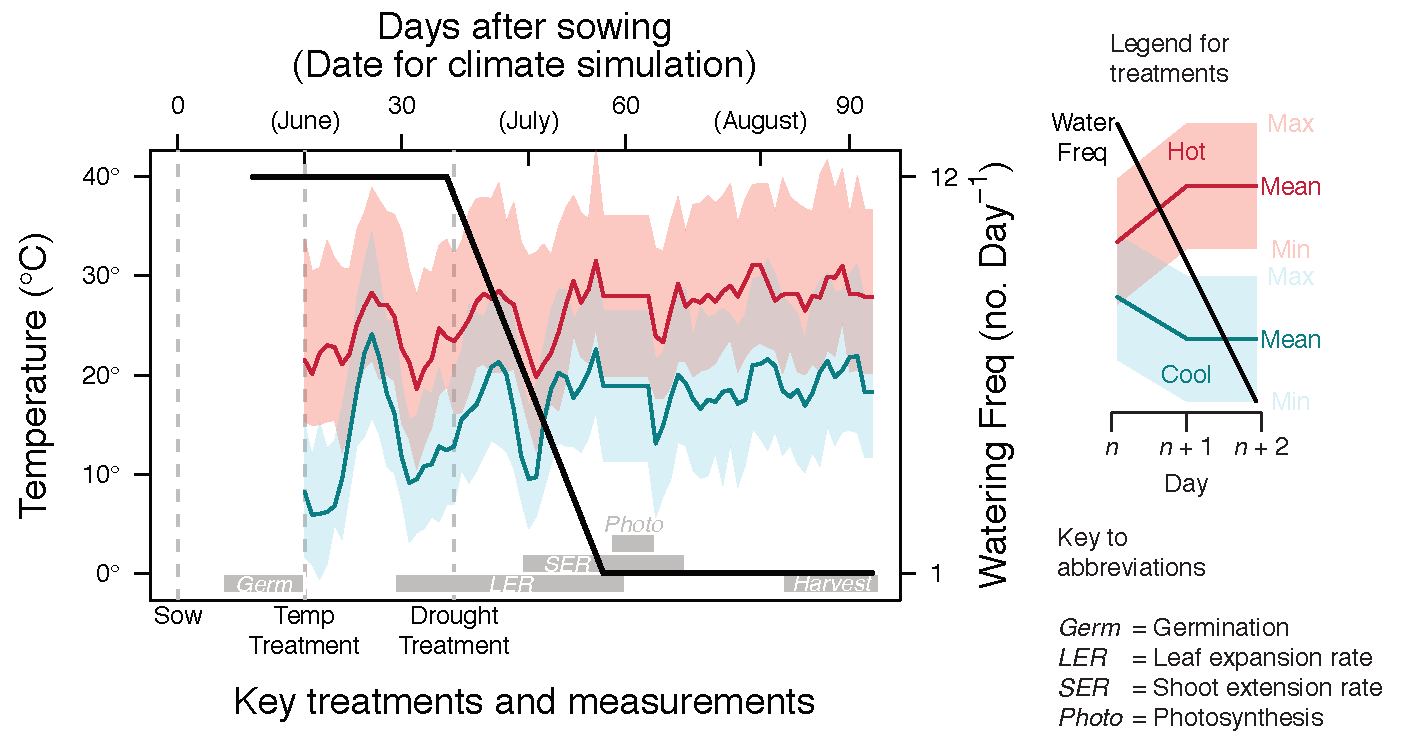
\includegraphics[width=1\textwidth]{Figures/Figure_ExptlDes.pdf}}
	\usefont{T1}{phv}{m}{n}
	\fontsize{10}{12}
	\selectfont
	\caption[Experimental Design]{CAPTION}
	\label{fig:Fig_ExptlDes}
\end{figure}

\subsection*{Growth and photosynthesis}

\begin{table}[ht]
   \centering
   \topcaption{Traits}
   \begin{tabular}{@{} ll @{}}
      \toprule
  Trait & Units \\
      \midrule
  Day of germination  & day \\
  Leaf expansion rate  &  mm day$^{-1}$  \\
  Shoot elongation rate  &  mm or cm day$^{-1}$  \\
  Harvest dry mass &  g  \\
  Photosynthetic rate &  $\mu$mol CO$_2$ m$^{-2}$ s$^{-1}$\\
  Mortality &  Probability?  \\
	    \bottomrule
   \end{tabular}
   \label{table:Table_traits}
\end{table}

\paragraph{Day of germination} We tested for population variation in germination rate, measured as Days to Germination, using a lognormal survival model fit using the survreg function in the R package \pkg{survival} version 2.38 \citep{Therneau_2015}. The model was fit with Population as a fixed effect and Family as random effect using a $\Gamma$ frailty function. The signifcance of the Population effect was determined using analysis of deviance.

\begin{knitrout}
\definecolor{shadecolor}{rgb}{0.969, 0.969, 0.969}\color{fgcolor}\begin{kframe}
\begin{alltt}
  \hlkwd{library}\hlstd{(survival)}
  \hlstd{pathMS} \hlkwb{<-} \hlstr{"~/Google Drive/CardLocalAdaptation/ms"}
  \hlstd{pathDat} \hlkwb{<-} \hlkwd{paste}\hlstd{(pathMS,} \hlstr{"/Data"}\hlstd{,} \hlkwc{sep} \hlstd{=} \hlstr{""}\hlstd{)}

  \hlstd{master} \hlkwb{<-} \hlkwd{read.csv}\hlstd{(}\hlkwd{paste}\hlstd{(pathDat,} \hlstr{"/MasterDatasheet_out.csv"}\hlstd{,} \hlkwc{sep} \hlstd{=} \hlstr{""}\hlstd{),}
    \hlkwc{row.names} \hlstd{=} \hlnum{1}\hlstd{)}

  \hlcom{# Create Surv object}
        \hlstd{germ} \hlkwb{<-} \hlkwd{with}\hlstd{(}\hlkwd{subset}\hlstd{(master,} \hlopt{!}\hlkwd{is.na}\hlstd{(master}\hlopt{$}\hlstd{MinGermDay)),} \hlkwd{Surv}\hlstd{(MinGermDay, MaxGermDay,}
                \hlkwc{type} \hlstd{=} \hlstr{"interval2"}\hlstd{))}

        \hlcom{# lognormal produced best fit to data}
        \hlstd{fitGerm} \hlkwb{<-} \hlkwd{survreg}\hlstd{(germ} \hlopt{~} \hlstd{PopID} \hlopt{+} \hlkwd{frailty}\hlstd{(Family,} \hlkwc{sparse} \hlstd{= F),}
                \hlkwc{data} \hlstd{=} \hlkwd{subset}\hlstd{(master,} \hlopt{!}\hlkwd{is.na}\hlstd{(master}\hlopt{$}\hlstd{MinGermDay)),} \hlkwc{dist} \hlstd{=} \hlstr{"lognormal"}\hlstd{)}
        \hlkwd{suppressWarnings}\hlstd{(}\hlkwd{anova}\hlstd{(fitGerm))} \hlcom{# significant family and population effects}
\end{alltt}
\begin{verbatim}
##                                   Df Deviance Resid. Df    -2*LL
## NULL                              NA       NA  700.0000 2796.417
## PopID                        15.0000 151.9495  685.0000 2644.468
## frailty(Family, sparse = F) 106.9738 254.7233  578.0262 2389.745
##                                 Pr(>Chi)
## NULL                                  NA
## PopID                       9.887489e-25
## frailty(Family, sparse = F) 4.530519e-14
\end{verbatim}
\end{kframe}
\end{knitrout}

\paragraph{Growth rate: leaf expansion and shoot elongation}

We censused longest leaf length $>1$ mm on 10 days (twice per week) between 12 May and 12 June (28 to 59 days after sowing). We ceased measuring leaf length once it appeared to asymptote and growth shifted to shoot elongation.  We also censused plant height on 7 days (twice per week) between 29 May and 20 June (45 to 67 days after sowing). Both leaf expansion and shoot elongation were modeled as a second-order polynomials of time with individual coefficients (separate for leaf and shoot growth) using empirical Bayes' estimates from linear mixed-effects models fit using the R package \pkg{lme4} version 1.1-7 \citep{Bates_etal_2014}.

\begin{knitrout}
\definecolor{shadecolor}{rgb}{0.969, 0.969, 0.969}\color{fgcolor}\begin{kframe}
\begin{alltt}
  \hlkwd{library}\hlstd{(lme4)}
\end{alltt}


{\ttfamily\noindent\itshape\color{messagecolor}{\#\# Loading required package: Matrix\\\#\# Loading required package: Rcpp}}\begin{alltt}
  \hlkwd{library}\hlstd{(lmerTest)}
\end{alltt}


{\ttfamily\noindent\itshape\color{messagecolor}{\#\# \\\#\# Attaching package: 'lmerTest'\\\#\# \\\#\# The following object is masked from 'package:lme4':\\\#\# \\\#\#\ \ \ \  lmer\\\#\# \\\#\# The following object is masked from 'package:stats':\\\#\# \\\#\#\ \ \ \  step}}\begin{alltt}
  \hlcom{# New (blank) datasheet on which to add data}
  \hlstd{newdata} \hlkwb{<-} \hlkwd{read.csv}\hlstd{(}\hlkwd{paste}\hlstd{(pathDat,} \hlstr{"/MasterDatasheet_in.csv"}\hlstd{,} \hlkwc{sep} \hlstd{=} \hlstr{""}\hlstd{))}

  \hlcom{# Read in LER data}
  \hlstd{LERdata} \hlkwb{<-} \hlkwd{read.csv}\hlstd{(}\hlkwd{paste}\hlstd{(pathDat,} \hlstr{"/LERdata.csv"}\hlstd{,} \hlkwc{sep} \hlstd{=} \hlstr{""}\hlstd{))}

  \hlcom{#}
        \hlcom{# Empirical Bayes Approach: get coefficients for every plant}
        \hlcom{#}

        \hlcom{# suppressWarnings(mmLER <- lmer(log(LLL) ~ poly(DayN, 2, raw = T) + }
    \hlcom{# (poly(DayN, 2, raw = T)|indiv), data = LERdata))}
  \hlcom{# save(mmLER, file = paste(pathDat, "/mmLER.RData", sep = ""))}
  \hlkwd{load}\hlstd{(}\hlkwc{file} \hlstd{=} \hlkwd{paste}\hlstd{(pathDat,} \hlstr{"/mmLER.RData"}\hlstd{,} \hlkwc{sep} \hlstd{=} \hlstr{""}\hlstd{))}

  \hlcom{# Extract coefficients and add to datasheet}
        \hlstd{Y} \hlkwb{<-} \hlkwd{t}\hlstd{(}\hlkwd{unlist}\hlstd{(}\hlkwd{fixef}\hlstd{(mmLER))} \hlopt{+} \hlkwd{t}\hlstd{(}\hlkwd{ranef}\hlstd{(mmLER)}\hlopt{$}\hlstd{indiv))[}\hlkwd{match}\hlstd{(newdata}\hlopt{$}\hlstd{indiv,}
                \hlkwd{rownames}\hlstd{(}\hlkwd{ranef}\hlstd{(mmLER)}\hlopt{$}\hlstd{indiv)), ]}
        \hlkwd{colnames}\hlstd{(Y)} \hlkwb{<-} \hlkwd{c}\hlstd{(}\hlstr{"b0_LER"}\hlstd{,} \hlstr{"b1_LER"}\hlstd{,} \hlstr{"b2_LER"}\hlstd{)}
  \hlstd{newdata} \hlkwb{<-} \hlkwd{cbind}\hlstd{(newdata, Y)}

  \hlcom{# Model-based LER}
        \hlcom{# Timeframe for Cool treatment: Day 0 - 31}
        \hlcom{# Timeframe for Hot treatment: Day 0 - 24}
        \hlstd{newdata}\hlopt{$}\hlstd{LERstart} \hlkwb{<-} \hlkwd{exp}\hlstd{(newdata}\hlopt{$}\hlstd{b0_LER)}
        \hlstd{newdata}\hlopt{$}\hlstd{LERend} \hlkwb{<-} \hlkwd{exp}\hlstd{(newdata}\hlopt{$}\hlstd{b0_LER} \hlopt{+}
                                        \hlstd{newdata}\hlopt{$}\hlstd{b1_LER} \hlopt{*} \hlkwd{ifelse}\hlstd{(newdata}\hlopt{$}\hlstd{TempTrt} \hlopt{==} \hlstr{"Cool"}\hlstd{,} \hlnum{31}\hlstd{,} \hlnum{24}\hlstd{)} \hlopt{+}
                                        \hlstd{newdata}\hlopt{$}\hlstd{b2_LER} \hlopt{*} \hlkwd{ifelse}\hlstd{(newdata}\hlopt{$}\hlstd{TempTrt} \hlopt{==} \hlstr{"Cool"}\hlstd{,} \hlnum{31} \hlopt{^} \hlnum{2}\hlstd{,} \hlnum{24} \hlopt{^} \hlnum{2}\hlstd{))}
        \hlstd{newdata}\hlopt{$}\hlstd{LER_AbsGrowth} \hlkwb{<-} \hlstd{(newdata}\hlopt{$}\hlstd{LERend} \hlopt{-} \hlstd{newdata}\hlopt{$}\hlstd{LERstart)} \hlopt{/}
                \hlkwd{ifelse}\hlstd{(newdata}\hlopt{$}\hlstd{TempTrt} \hlopt{==} \hlstr{"Cool"}\hlstd{,} \hlnum{31}\hlstd{,} \hlnum{24}\hlstd{)}

  \hlcom{# Mixed model ANOVA with family as random factor fit using step down procedure}
        \hlstd{mm} \hlkwb{<-} \hlkwd{lmer}\hlstd{(LER_AbsGrowth} \hlopt{~} \hlstd{AvgGermDay} \hlopt{+} \hlstd{PopID} \hlopt{*} \hlstd{TempTrt} \hlopt{*} \hlstd{WaterTrt} \hlopt{+} \hlstd{(}\hlnum{1}\hlopt{|}\hlstd{Family),}
                \hlkwc{data} \hlstd{= master)}
        \hlstd{fitLER} \hlkwb{<-} \hlkwd{step}\hlstd{(mm,} \hlkwc{reduce.random} \hlstd{= F)} \hlcom{# includes pop, temp, h2o, population x water}
        \hlcom{# fitLER <- step(mm, ddf = "Kenward-Roger", reduce.random = F) # same result using Satterthwaite ddf}
\end{alltt}
\end{kframe}
\end{knitrout}


\begin{knitrout}
\definecolor{shadecolor}{rgb}{0.969, 0.969, 0.969}\color{fgcolor}\begin{kframe}
\begin{alltt}
  \hlcom{# Read in SER data}
  \hlstd{SERdata} \hlkwb{<-} \hlkwd{read.csv}\hlstd{(}\hlkwd{paste}\hlstd{(pathDat,} \hlstr{"/SERdata.csv"}\hlstd{,} \hlkwc{sep} \hlstd{=} \hlstr{""}\hlstd{))}

  \hlcom{#}
  \hlcom{# Empirical Bayes Approach: get coefficients for every plant}
        \hlcom{#}

        \hlcom{# suppressWarnings(mmSER <- lmer(log(height + 1) ~ poly(DayN, 2, raw = T) + }
    \hlcom{# (poly(DayN, 2, raw = T)|indiv), data = SERdata))}
  \hlcom{# save(mmSER, file = paste(pathDat, "/mmSER.RData", sep = ""))}
  \hlkwd{load}\hlstd{(}\hlkwc{file} \hlstd{=} \hlkwd{paste}\hlstd{(pathDat,} \hlstr{"/mmSER.RData"}\hlstd{,} \hlkwc{sep} \hlstd{=} \hlstr{""}\hlstd{))}

  \hlcom{# Extract coefficients and add to datasheet}
  \hlstd{Y} \hlkwb{<-} \hlkwd{t}\hlstd{(}\hlkwd{unlist}\hlstd{(}\hlkwd{fixef}\hlstd{(mmSER))} \hlopt{+} \hlkwd{t}\hlstd{(}\hlkwd{ranef}\hlstd{(mmSER)}\hlopt{$}\hlstd{indiv))[}\hlkwd{match}\hlstd{(newdata}\hlopt{$}\hlstd{indiv,}
                \hlkwd{rownames}\hlstd{(}\hlkwd{ranef}\hlstd{(mmSER)}\hlopt{$}\hlstd{indiv)), ]}
        \hlkwd{colnames}\hlstd{(Y)} \hlkwb{<-} \hlkwd{c}\hlstd{(}\hlstr{"b0_SER"}\hlstd{,} \hlstr{"b1_SER"}\hlstd{,} \hlstr{"b2_SER"}\hlstd{)}
  \hlstd{newdata} \hlkwb{<-} \hlkwd{cbind}\hlstd{(newdata, Y)}

  \hlcom{# Model-based SER}
        \hlcom{# Timeframe for Cool treatment: Day 0 - 31}
        \hlcom{# Timeframe for Hot treatment: Day 0 - 24}
        \hlstd{newdata}\hlopt{$}\hlstd{SERstart} \hlkwb{<-} \hlkwd{exp}\hlstd{(newdata}\hlopt{$}\hlstd{b0_SER)}
        \hlstd{newdata}\hlopt{$}\hlstd{SERend} \hlkwb{<-} \hlkwd{exp}\hlstd{(newdata}\hlopt{$}\hlstd{b0_SER} \hlopt{+}
                                        \hlstd{newdata}\hlopt{$}\hlstd{b1_SER} \hlopt{*} \hlkwd{ifelse}\hlstd{(newdata}\hlopt{$}\hlstd{TempTrt} \hlopt{==} \hlstr{"Cool"}\hlstd{,} \hlnum{31}\hlstd{,} \hlnum{24}\hlstd{)} \hlopt{+}
                                        \hlstd{newdata}\hlopt{$}\hlstd{b2_SER} \hlopt{*} \hlkwd{ifelse}\hlstd{(newdata}\hlopt{$}\hlstd{TempTrt} \hlopt{==} \hlstr{"Cool"}\hlstd{,} \hlnum{31} \hlopt{^} \hlnum{2}\hlstd{,} \hlnum{24} \hlopt{^} \hlnum{2}\hlstd{))}
        \hlstd{newdata}\hlopt{$}\hlstd{SER_AbsGrowth} \hlkwb{<-} \hlstd{(newdata}\hlopt{$}\hlstd{SERend} \hlopt{-} \hlstd{newdata}\hlopt{$}\hlstd{SERstart)} \hlopt{/}
                \hlkwd{ifelse}\hlstd{(newdata}\hlopt{$}\hlstd{TempTrt} \hlopt{==} \hlstr{"Cool"}\hlstd{,} \hlnum{31}\hlstd{,} \hlnum{24}\hlstd{)}

  \hlstd{mm} \hlkwb{<-} \hlkwd{lmer}\hlstd{(SER_AbsGrowth} \hlopt{~} \hlstd{AvgGermDay} \hlopt{+} \hlstd{PopID} \hlopt{*} \hlstd{TempTrt} \hlopt{*} \hlstd{WaterTrt} \hlopt{+}
                \hlstd{(}\hlnum{1}\hlopt{|}\hlstd{Family),} \hlkwc{data} \hlstd{= master)}
        \hlstd{fitSER} \hlkwb{<-} \hlkwd{step}\hlstd{(mm,} \hlkwc{reduce.random} \hlstd{= F)} \hlcom{#includes pop, temp, h2o, temp x water}
\end{alltt}
\end{kframe}
\end{knitrout}

\paragraph{Photosynthesis}
During the week of 10 to 16 June (57 to 63 days after sowing), we measured daytime photosynthetic rate and stomatal conductance on a subset of 329 plants evenly spread between treatments and families within populations. The youngest, fully-expanded leaf acclimated for 3 minutes to reach steady state in a 6 cm$^2$ chamber of a LI-COR 6400XT Portable Photosynthesis System (LI-COR Biosciences, Lincoln, Nebraska). All measurements were made at ambient light (400 $\mu$mol m$^{-2}$ s$^{-1}$), temperature, and moderate relative humidity. During this period, we suspended normal day-to-day temperature fluctuations and set daytime temperatures to its average for that period (Cool: 26.5$\degree$; Hot: 36.1$\degree$ \cdm{get exact temps used}) so that all plants within a temperature treatment were measured under the same conditions.

\begin{knitrout}
\definecolor{shadecolor}{rgb}{0.969, 0.969, 0.969}\color{fgcolor}\begin{kframe}
\begin{alltt}
  \hlcom{# Photosynthetic rate}
  \hlstd{mm} \hlkwb{<-} \hlkwd{lmer}\hlstd{(Photo} \hlopt{~} \hlstd{PopID} \hlopt{*} \hlstd{TempTrt} \hlopt{*} \hlstd{WaterTrt} \hlopt{+} \hlstd{(}\hlnum{1}\hlopt{|}\hlstd{Family),}
    \hlkwc{data} \hlstd{=} \hlkwd{subset}\hlstd{(master,} \hlopt{!}\hlkwd{is.na}\hlstd{(master}\hlopt{$}\hlstd{Photo)))}
  \hlstd{fitPhoto} \hlkwb{<-} \hlkwd{step}\hlstd{(mm,} \hlkwc{reduce.random} \hlstd{= F)}

  \hlcom{# Intrinsic photosynthetic rate}
  \hlcom{# = residuals of Conductance - Photosynthesis regression}
  \hlcom{# Removed one outlier (may change if data are rearranged!)}
        \hlstd{mm} \hlkwb{<-} \hlkwd{lmer}\hlstd{(resPhoto} \hlopt{~} \hlstd{PopID} \hlopt{*} \hlstd{TempTrt} \hlopt{*} \hlstd{WaterTrt} \hlopt{+} \hlstd{(}\hlnum{1}\hlopt{|}\hlstd{Family),}
    \hlkwc{data} \hlstd{=} \hlkwd{subset}\hlstd{(master,} \hlopt{!}\hlkwd{is.na}\hlstd{(master}\hlopt{$}\hlstd{Photo))[}\hlopt{-}\hlnum{52}\hlstd{, ])}
        \hlstd{fitIntrnPhoto} \hlkwb{<-} \hlkwd{step}\hlstd{(mm,} \hlkwc{reduce.random} \hlstd{= F)}
\end{alltt}
\end{kframe}
\end{knitrout}

\paragraph{Mortality}
We assayed mortality during twice-weekly growth measurements. We could not get GLMM with Family effects to converge, so we used GLM with a quasibinomial error structure and assessed signifiance using Type 2 Analysis of Deviance with the R package \pkg{car}. 

\begin{knitrout}
\definecolor{shadecolor}{rgb}{0.969, 0.969, 0.969}\color{fgcolor}\begin{kframe}
\begin{alltt}
  \hlkwd{library}\hlstd{(car)}

  \hlstd{fitMort} \hlkwb{<-} \hlkwd{glm}\hlstd{(DiedFromStress} \hlopt{~} \hlstd{PopID} \hlopt{*} \hlstd{TempTrt} \hlopt{*} \hlstd{WaterTrt,}
    \hlkwc{data} \hlstd{=} \hlkwd{subset}\hlstd{(master,} \hlopt{!}\hlkwd{is.na}\hlstd{(master}\hlopt{$}\hlstd{DiedFromStress)),} \hlkwc{family} \hlstd{=} \hlstr{"quasibinomial"}\hlstd{)}

  \hlkwd{Anova}\hlstd{(fitMort,} \hlkwc{type} \hlstd{=} \hlnum{2}\hlstd{)}
\end{alltt}
\begin{verbatim}
## Analysis of Deviance Table (Type II tests)
## 
## Response: DiedFromStress
##                        LR Chisq Df Pr(>Chisq)    
## PopID                    38.169 15  0.0008519 ***
## TempTrt                 247.763  1  < 2.2e-16 ***
## WaterTrt                 79.508  1  < 2.2e-16 ***
## PopID:TempTrt            26.188 15  0.0360962 *  
## PopID:WaterTrt           11.547 15  0.7129658    
## TempTrt:WaterTrt         48.543  1  3.231e-12 ***
## PopID:TempTrt:WaterTrt    8.685 15  0.8934160    
## ---
## Signif. codes:  0 '***' 0.001 '**' 0.01 '*' 0.05 '.' 0.1 ' ' 1
\end{verbatim}
\end{kframe}
\end{knitrout}

\paragraph{Biomass (show correlation between growth rate and biomass?)}

\subsection*{Intrinsic variation and plasticity}

For all traits (Table~\ref{table:Table_traits}) we tested for Population, Treatment, and Population $\times$ Treatment interactions. We interpreted significant Population effects to indicate intrinsic variation and Population by Treatment effects to indicate variation in plasticity. As mentioned above, we survival and GLM models for germination rate and mortality, respectively. For all other traits, we used mixed model ANOVAs with Family included as a random factor. Models were fit by restricted maximum likelihood using lmer from the R package \pkg{lme4} \citep{Bates_etal_2014}. Significant fixed effect terms were selected using a step-wise backward elimination procedure implemented with the step function in the R package \pkg{lmerTest} version 2.0-11 \citep{Kuznetsova_etal_2014}. Denominator degrees of freedom for $F$-tests were estimated using Satterthwaite's approximation. Significant Population effect indicate intrinsic trait differences; significant Population $\times$ Treatment effects indicate population differences in plasticity. For growth rate, we also accounted for differences in germination rate by including day of germination as a factor.

\subsection*{Principal components of germination, growth, and photosynthesis}
[maybe this goes in Results?]
We summarized population-level coefficients, after factoring out Treatment and other effects, using principal components. 
\begin{knitrout}
\definecolor{shadecolor}{rgb}{0.969, 0.969, 0.969}\color{fgcolor}\begin{kframe}
\begin{alltt}
  \hlstd{popMeans} \hlkwb{<-} \hlkwd{data.frame}\hlstd{(}
    \hlkwc{germ} \hlstd{=} \hlkwd{c}\hlstd{(}\hlkwd{coef}\hlstd{(fitGerm)[}\hlnum{1}\hlstd{],} \hlkwd{coef}\hlstd{(fitGerm)[}\hlnum{1}\hlstd{]} \hlopt{+} \hlkwd{coef}\hlstd{(fitGerm)[}\hlnum{2}\hlopt{:}\hlnum{16}\hlstd{]),}
    \hlkwc{LER} \hlstd{= fitLER}\hlopt{$}\hlstd{lsmeans.table[}\hlnum{1}\hlopt{:}\hlnum{16}\hlstd{,} \hlstr{"Estimate"}\hlstd{],}
    \hlkwc{SER} \hlstd{= fitSER}\hlopt{$}\hlstd{lsmeans.table[}\hlnum{1}\hlopt{:}\hlnum{16}\hlstd{,} \hlstr{"Estimate"}\hlstd{],}
    \hlkwc{photo} \hlstd{= fitIntrnPhoto}\hlopt{$}\hlstd{lsmeans.table[}\hlnum{1}\hlopt{:}\hlnum{16}\hlstd{,} \hlstr{"Estimate"}\hlstd{])}

  \hlstd{traitPC} \hlkwb{<-} \hlkwd{prcomp}\hlstd{(popMeans,} \hlkwc{center} \hlstd{= T,} \hlkwc{scale.} \hlstd{= T)}
  \hlstd{focClim}\hlopt{$}\hlstd{PC1} \hlkwb{<-} \hlstd{traitPC}\hlopt{$}\hlstd{x[,} \hlstr{"PC1"}\hlstd{]}
  \hlstd{focClimSA}\hlopt{$}\hlstd{PC1} \hlkwb{<-} \hlstd{traitPC}\hlopt{$}\hlstd{x[,} \hlstr{"PC1"}\hlstd{]}

  \hlcom{# Percent variance explained by first principal component}
  \hlstd{pve} \hlkwb{<-} \hlkwd{paste}\hlstd{(}\hlkwd{round}\hlstd{(}\hlnum{100} \hlopt{*} \hlstd{traitPC}\hlopt{$}\hlstd{sdev[}\hlnum{1}\hlstd{]} \hlopt{^} \hlnum{2} \hlopt{/} \hlkwd{sum}\hlstd{(traitPC}\hlopt{$}\hlstd{sdev} \hlopt{^} \hlnum{2}\hlstd{),} \hlnum{1}\hlstd{),} \hlstr{"%"}\hlstd{)}

  \hlcom{# Plot latitude versus PC1}
  \hlkwd{pdf}\hlstd{(}\hlkwd{paste}\hlstd{(pathFig,} \hlstr{"/Figure_PC1vLat.pdf"}\hlstd{,} \hlkwc{sep} \hlstd{=} \hlstr{""}\hlstd{),} \hlnum{5.5}\hlstd{,} \hlnum{5}\hlstd{)}
  \hlkwd{par}\hlstd{(}\hlkwc{mai} \hlstd{=} \hlkwd{c}\hlstd{(}\hlnum{1}\hlstd{,} \hlnum{1.5}\hlstd{,} \hlnum{0.25}\hlstd{,} \hlnum{0.25}\hlstd{))}
  \hlkwd{plot}\hlstd{(focClim}\hlopt{$}\hlstd{Lat, focClim}\hlopt{$}\hlstd{PC1,} \hlkwc{xlim} \hlstd{=} \hlkwd{c}\hlstd{(}\hlnum{32}\hlstd{,} \hlnum{44}\hlstd{),} \hlkwc{ylim} \hlstd{=} \hlkwd{c}\hlstd{(}\hlopt{-}\hlnum{4}\hlstd{,} \hlnum{4}\hlstd{),} \hlkwc{axes} \hlstd{= F,}
    \hlkwc{frame.plot} \hlstd{= T,} \hlkwc{type} \hlstd{=} \hlstr{"n"}\hlstd{,} \hlkwc{xlab} \hlstd{=} \hlstr{""}\hlstd{,} \hlkwc{ylab} \hlstd{=} \hlstr{""}\hlstd{)}
  \hlkwd{title}\hlstd{(}\hlkwc{xlab} \hlstd{=} \hlstr{"Latitude"}\hlstd{,} \hlkwc{cex.lab} \hlstd{=} \hlnum{1.5}\hlstd{)}
  \hlkwd{title}\hlstd{(}\hlkwc{ylab} \hlstd{=} \hlkwd{substitute}\hlstd{(}\hlkwd{plain}\hlstd{(Principal}\hlopt{~}\hlstd{Component}\hlopt{~}\hlnum{1}\hlstd{)}\hlopt{~}\hlkwd{group}\hlstd{(}\hlstr{"("}\hlstd{, x,} \hlstr{")"}\hlstd{),}
    \hlkwd{list}\hlstd{(}\hlkwc{x} \hlstd{= pve)))}
  \hlkwd{axis}\hlstd{(}\hlnum{1}\hlstd{,} \hlkwc{at} \hlstd{=} \hlkwd{seq}\hlstd{(}\hlnum{32}\hlstd{,} \hlnum{44}\hlstd{,} \hlnum{4}\hlstd{),} \hlkwc{labels} \hlstd{=} \hlkwd{c}\hlstd{(}\hlkwd{expression}\hlstd{(}\hlnum{32}\hlopt{*}\hlstd{degree),}
                \hlkwd{expression}\hlstd{(}\hlnum{36}\hlopt{*}\hlstd{degree),} \hlkwd{expression}\hlstd{(}\hlnum{40}\hlopt{*}\hlstd{degree),} \hlkwd{expression}\hlstd{(}\hlnum{44}\hlopt{*}\hlstd{degree)),}
                \hlkwc{lwd} \hlstd{=} \hlnum{0}\hlstd{,} \hlkwc{lwd.ticks} \hlstd{=} \hlnum{1}\hlstd{)}
  \hlkwd{axis}\hlstd{(}\hlnum{2}\hlstd{,} \hlkwc{at} \hlstd{=} \hlkwd{seq}\hlstd{(}\hlopt{-}\hlnum{4}\hlstd{,} \hlnum{4}\hlstd{,} \hlnum{2}\hlstd{),} \hlkwc{las} \hlstd{=} \hlnum{1}\hlstd{,} \hlkwc{lwd} \hlstd{=} \hlnum{0}\hlstd{,} \hlkwc{lwd.ticks} \hlstd{=} \hlnum{1}\hlstd{)}
  \hlstd{fitLat} \hlkwb{<-} \hlkwd{lm}\hlstd{(PC1} \hlopt{~} \hlstd{Latitude,} \hlkwc{data} \hlstd{= focClim)}

        \hlcom{# Label y-axis from slow to fast growth}
        \hlkwd{mtext}\hlstd{(}\hlkwd{c}\hlstd{(}\hlstr{"Slow\textbackslash{}nGrowth"}\hlstd{,} \hlstr{"Fast\textbackslash{}nGrowth"}\hlstd{),} \hlnum{2}\hlstd{,} \hlkwc{at} \hlstd{=} \hlkwd{c}\hlstd{(}\hlopt{-}\hlnum{4}\hlstd{,} \hlnum{4}\hlstd{),} \hlkwc{cex} \hlstd{=} \hlnum{1.25}\hlstd{,}
                                \hlkwc{font} \hlstd{=} \hlnum{3}\hlstd{,} \hlkwc{las} \hlstd{=} \hlnum{1}\hlstd{,} \hlkwc{line} \hlstd{=} \hlnum{4}\hlstd{,} \hlkwc{adj} \hlstd{=} \hlnum{0.5}\hlstd{)}

  \hlcom{# polygon of confidence intervals}
  \hlstd{x} \hlkwb{<-} \hlkwd{seq}\hlstd{(}\hlkwd{min}\hlstd{(focClim}\hlopt{$}\hlstd{Latitude),} \hlkwd{max}\hlstd{(focClim}\hlopt{$}\hlstd{Latitude),} \hlkwc{l} \hlstd{=} \hlnum{1e3}\hlstd{)}
  \hlstd{u} \hlkwb{<-} \hlkwd{predict}\hlstd{(fitLat,} \hlkwc{new} \hlstd{=} \hlkwd{data.frame}\hlstd{(}\hlkwc{Latitude} \hlstd{= x))}
  \hlstd{s} \hlkwb{<-} \hlkwd{sqrt}\hlstd{(}\hlkwd{sapply}\hlstd{(x,} \hlkwa{function}\hlstd{(}\hlkwc{X}\hlstd{)} \hlkwd{t}\hlstd{(}\hlkwd{c}\hlstd{(}\hlnum{1}\hlstd{, X))} \hlopt \hlkwd{vcov}\hlstd{(fitLat)} \hlopt \hlkwd{c}\hlstd{(}\hlnum{1}\hlstd{, X)))}
  \hlstd{confInt} \hlkwb{<-} \hlkwd{data.frame}\hlstd{(}\hlkwc{lowerCI} \hlstd{=} \hlkwd{qnorm}\hlstd{(}\hlnum{0.025}\hlstd{, u, s),} \hlkwc{upperCI} \hlstd{=} \hlkwd{qnorm}\hlstd{(}\hlnum{0.975}\hlstd{, u, s))}
  \hlkwd{polygon}\hlstd{(}\hlkwd{c}\hlstd{(x,} \hlkwd{rev}\hlstd{(x)),} \hlkwd{c}\hlstd{(confInt}\hlopt{$}\hlstd{lowerCI,} \hlkwd{rev}\hlstd{(confInt}\hlopt{$}\hlstd{upperCI)),}
    \hlkwc{col} \hlstd{=} \hlstr{"grey80"}\hlstd{,} \hlkwc{border} \hlstd{=} \hlnum{NA}\hlstd{)}
  \hlkwd{lines}\hlstd{(x, confInt}\hlopt{$}\hlstd{lowerCI,} \hlkwc{lwd} \hlstd{=} \hlnum{2}\hlstd{,} \hlkwc{lty} \hlstd{=} \hlnum{2}\hlstd{)}
  \hlkwd{lines}\hlstd{(x, confInt}\hlopt{$}\hlstd{upperCI,} \hlkwc{lwd} \hlstd{=} \hlnum{2}\hlstd{,} \hlkwc{lty} \hlstd{=} \hlnum{2}\hlstd{)}
  \hlkwd{lines}\hlstd{(}\hlkwd{range}\hlstd{(focClim}\hlopt{$}\hlstd{Lat),} \hlkwd{rev}\hlstd{(}\hlkwd{range}\hlstd{(}\hlkwd{predict}\hlstd{(fitLat))),} \hlkwc{lwd} \hlstd{=} \hlnum{2}\hlstd{)}
  \hlkwd{points}\hlstd{(focClim}\hlopt{$}\hlstd{Lat, focClim}\hlopt{$}\hlstd{PC1,} \hlkwc{pch} \hlstd{=} \hlnum{21}\hlstd{,} \hlkwc{col} \hlstd{=} \hlstr{"black"}\hlstd{,} \hlkwc{bg} \hlstd{= primShade0,} \hlkwc{cex} \hlstd{=} \hlnum{1.5}\hlstd{,}
    \hlkwc{lwd} \hlstd{=} \hlnum{2}\hlstd{)}
  \hlkwd{dev.off}\hlstd{()}
\end{alltt}
\begin{verbatim}
## pdf 
##   2
\end{verbatim}
\begin{alltt}
  \hlcom{# plot axes could be range maps with areas highlighted (x-axis) and short to tall plants (y-axis)}
  \hlcom{#plot(focClim$Lat, traitPC$x[, "PC1"])}
  \hlcom{#cor.test(focClim$Lat, traitPC$x[, "PC1"])}
  \hlcom{#cor.test(popMeans[, 4], traitPC$x[, "PC1"])}
  \hlcom{#plot(focClim$bio16_cva, traitPC$x[, "PC1"])}
\end{alltt}
\end{kframe}
\end{knitrout}

\begin{knitrout}
\definecolor{shadecolor}{rgb}{0.969, 0.969, 0.969}\color{fgcolor}\begin{kframe}
\begin{alltt}
\hlcom{# R data.frame of 178 M. cardinalis occurrences, thinned to correct for sampling bias, and associated climate data}
\hlkwd{load}\hlstd{(}\hlkwd{paste}\hlstd{(pathDat,} \hlstr{"/thinnedOccClimate.RData"}\hlstd{,} \hlkwc{sep} \hlstd{=} \hlstr{""}\hlstd{))}
\end{alltt}
\end{kframe}
\end{knitrout}



